\chapter{Algorithm for test}
\label{cha:bacAlg}

In this chapter we present the bacteriological algorithm, used to generate and
select the job configurations for Hadoop. 

\section{Genetic Algorithm}
\label{subsec:evolutionay_algorithms}
Evolutionary Algorithms are inspired on biological evolution process to select
the best inviduals that adapt themselves in the environment. For this adptation
is mimicked biological mechanisms such as \textbf{reproduction}, \textbf{mutation},
\textbf{recombination or crossover} and \textbf{selection}. One of the most known
evolutionary algorithms is the Genetic Algorithm(GA).

On GA context there are three important components:
\begin{itemize}
    \item \textbf{Gene} that is the smaller particle.
    \item \textbf{Individual} that is composed for genes.
    \item \textbf{Population} that is composed for individuals.
\end{itemize}

The GA works on the gene level, so all changes are done in this level. At first
glance, changes done on gene seems tiny and without much relevance, but them can
be crucial for adaptation of the individual in the environment, also genetic
changes can be crucial to survival of one entire population or even mean survival
of a species.

%Rosenzweig~\cite{rosenzweig:1995} cites that in the evolution
%process barriers may exist, like geographical barrier retricts gene flow within
%a sexually reproducing population and these genes could define the existence another
%population.

The GA process describe in Figure~\ref{fig:ga} has its main strategy
based in tree biological mechanisms: \textbf{reproduction}, \textbf{crossover}
and \textbf{mutation} which are further detailed below:

\begin{itemize}
	\item \textbf{Reproduction}: copies the individuals to participe of the next
	stage (the crossover), they are chosen based on their abilities in adapt themselves
	to the environment. Those abilities can be calculated according with a function
	\textit{F(x)} that is called as the fitness of the individual like described
	in Figure~\ref{fig:ga}.

    The choice of one individual is based in your fitness, it is similar to spin
    a roulette wheel where each individual receive slots according
    with your fitness, e.g. if an individual has F(X) = 10, then it has 10 slots
    in the roulette and suppose it has 100 slots, so the chance to choose this individual
    to participate in crossover is {\it100 slots / F(X) = 1/10}. Thus the individual
    fitness is greater, then your number of copies tends to be greater.

	\item \textbf{Crossover}: the crossover is similar the natural process called
	chromosomal crossover. This process is based on genetic recombination of
	chromosomes	to produce new genetic combinations. Basically the genes of two
    individuals are genetically combined to generate another resultant individual,
    so the new individual has some characteristics of both parent.
	More minutely in the genetic algorithm two individuals are chosen randomly {\bf(A, B)},
	an integer k, between 0 and the size {\it n} of an individual less one, is chosen
	randomly. The new individual {\it A'} is composed by the first {\it k} genes of A
	and the last {\it k - n} genes of B. The individual {\it B'} consists of the
	first {\it k} genes of B and the last {\it k - n} genes of A. 

	\item \textbf{Mutation}: after the crossover stage one mutation occur in the
	genes of new individuals. The natural process consist basically in change enzymes
    or proteins of genes in order to create new individual. The process on GA is
    simple in which one or more genes are selected randomly and then are changed
    (e.g. change one or more nucleotides of the DNA	of one chromosome).

% or one gene is constituted for bits 0 or 1 and one bit is
%	changed from 0 to 1).
\end{itemize}

\begin{figure}[htbp]
	\centering
	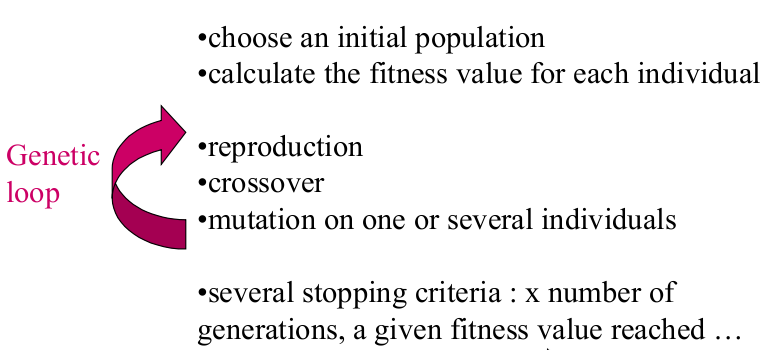
\includegraphics[width=\columnwidth]{img/ga.png}
	\caption{Genetic Algotithm process - Figure extracted from~\cite{baudry}.}\label{fig:ga}
\end{figure}

The algorithm begins with an initial population, for each individual is calculated
your fitness that is the base for reproduction mechanism, so the three biological
mechanisms is called in the specific order already detailed and so the resultant
population is evaluated as one or more criteria, if necessary the three mechanism
are run again and the process continues until the criteria to be achieved.

\section{Bacteriological Algorithm}

The bacteriological algorithm is part of the family of genetic algorithms that
works on genetic context. A minor particle this algorithm is a gene, but without
minor importance, all changes are influenced by it. The genes when clustered form
an individual that have more representativeness than an gene and the top is the
population that is set of individuals.

Compared to GA the Bacteriological Algorithm(BA) the individual is one bacteria
and the focus of the algorithm is to adapt itself in a given specific environment.
The algotithm is more one adaptive approach of GA than one otimization, but it have
some peculiarities that improve some issues involving the GA and change your behavior.

BA introduces a new mechanism called memorization that is responsable for memorize
the best individuals created along the generations. As described in~\cite{baudry},
it was proposed to improve the convergence of the GA, the introduction of the new
mechanism might appear one small modification, but actually reflects one crucial
change on GA's.

Besides of the introduction the new mechanism, the crossover mechanism was
removed because of the bacteria behavior on its adaptation process in the
environment. This mechanism cannot be used anymore, in terms of natural bacteriologic
process the remotion of the crossover make sense, the bacteria reproduce themself
asexually, consequently there is not crossover between two individuals, because
the reproduction process consist in duplication of DNA of one bacterium and after
a division to form two new bacteria.

The algorithm in high-level of abstraction is described in Figure~\ref{fig:ga}.
The BA is started and has four main mechanisms: {\bf Fitness computation}, {\bf Memorization},
{\bf Reproduction} and {\bf Mutation} which are detailed below:

\begin{itemize}
	\item Fitness computation: the fitness analogously to GA is one way to 	
	differentiate the abilities of each individual in adapt themselves to the
	environment. Calculation depends on several criteria defined by 
	the programer and is used to select the best individuals for the next generation.

	\item Memorization: is the main mechanism introduced by the BA. Its is responsable
	for memorizing the best individuals generated by the process of adaptation,
	as the process continues, the population improve more quickly its capacity of
	adaptation. The process consist in memorize the best individuals through 
	the	generations, if one generation generates bad individuals, i.e. generate low
	fitness values, then the memorization operator ignores this generation and
	uses the best individuals from past generations to the next generation in order
	to avoid regressions in the process.

	\item Reproduction: is similar to GA, the best individuals are sorted randomly
	and selected to the mutation process. One drawback in this stage is the population
    size can grow up exponentially, so thresholds must be established.

	\item Mutation: this stage is responsible for generating new individuals, one
	or several genes are changed in order to improve the adaptation of the bacteria
	population to the environment. These new individuals are evaluated by their
	fitness and they may be inserted in the set of best	individuals.

\end{itemize}

\begin{figure}[htbp]
	\centering
	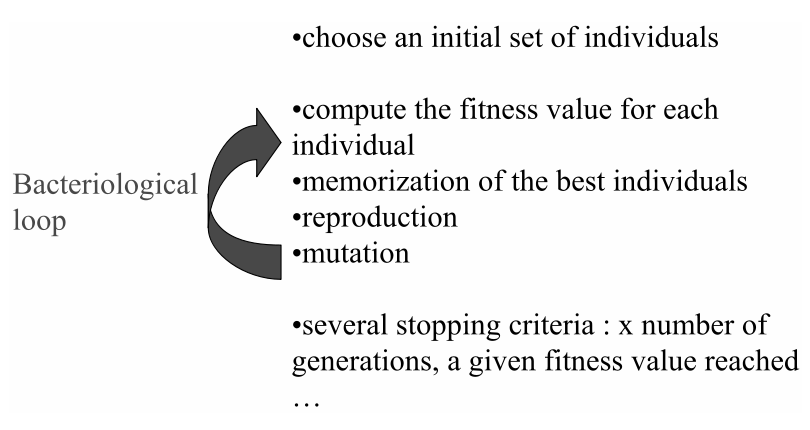
\includegraphics[width=\columnwidth]{img/ba.png}
	\caption{Bacteriological Algotithm process - Figure extracted from~\cite{baudry}.}\label{fig:ba}
\end{figure}

